\documentclass{article}

% if you need to pass options to natbib, use, e.g.:
%     \PassOptionsToPackage{numbers, compress}{natbib}
% before loading neurips_2025

% The authors should use one of these tracks.
% Before accepting by the NeurIPS conference, select one of the options below.
% 0. "default" for submission
 \usepackage[main, final]{neurips_2025}
% the "default" option is equal to the "main" option, which is used for the Main Track with double-blind reviewing.
% 1. "main" option is used for the Main Track
%  \usepackage[main]{neurips_2025}
% 2. "position" option is used for the Position Paper Track
%  \usepackage[position]{neurips_2025}
% 3. "dandb" option is used for the Datasets & Benchmarks Track
 % \usepackage[dandb]{neurips_2025}
% 4. "creativeai" option is used for the Creative AI Track
%  \usepackage[creativeai]{neurips_2025}
% 5. "sglblindworkshop" option is used for the Workshop with single-blind reviewing
 % \usepackage[sglblindworkshop]{neurips_2025}
% 6. "dblblindworkshop" option is used for the Workshop with double-blind reviewing
%  \usepackage[dblblindworkshop]{neurips_2025}

% After being accepted, the authors should add "final" behind the track to compile a camera-ready version.
% 1. Main Track
 % \usepackage[main, final]{neurips_2025}
% 2. Position Paper Track
%  \usepackage[position, final]{neurips_2025}
% 3. Datasets & Benchmarks Track
 % \usepackage[dandb, final]{neurips_2025}
% 4. Creative AI Track
%  \usepackage[creativeai, final]{neurips_2025}
% 5. Workshop with single-blind reviewing
%  \usepackage[sglblindworkshop, final]{neurips_2025}
% 6. Workshop with double-blind reviewing
%  \usepackage[dblblindworkshop, final]{neurips_2025}
% Note. For the workshop paper template, both \title{} and \workshoptitle{} are required, with the former indicating the paper title shown in the title and the latter indicating the workshop title displayed in the footnote.
% For workshops (5., 6.), the authors should add the name of the workshop, "\workshoptitle" command is used to set the workshop title.
% \workshoptitle{WORKSHOP TITLE}

% "preprint" option is used for arXiv or other preprint submissions
 % \usepackage[preprint]{neurips_2025}

% to avoid loading the natbib package, add option nonatbib:
%    \usepackage[nonatbib]{neurips_2025}

\usepackage[utf8]{inputenc} % allow utf-8 input
\usepackage[T1]{fontenc}    % use 8-bit T1 fonts
\usepackage{hyperref}       % hyperlinks
\usepackage{url}            % simple URL typesetting
\usepackage{booktabs}       % professional-quality tables
\usepackage{amsfonts}       % blackboard math symbols
\usepackage{nicefrac}       % compact symbols for 1/2, etc.
\usepackage{microtype}      % microtypography
\usepackage{xcolor}         % colors
\usepackage{minted}         % syntax highlighting for code
\usepackage{graphicx}       % include graphics
\usepackage{subcaption}     % subfigures

% Note. For the workshop paper template, both \title{} and \workshoptitle{} are required, with the former indicating the paper title shown in the title and the latter indicating the workshop title displayed in the footnote. 
\title{Diagnosing the Memory Throughput Bottleneck in the Era of Neural Rendering}


% The \author macro works with any number of authors. There are two commands
% used to separate the names and addresses of multiple authors: \And and \AND.
%
% Using \And between authors leaves it to LaTeX to determine where to break the
% lines. Using \AND forces a line break at that point. So, if LaTeX puts 3 of 4
% authors names on the first line, and the last on the second line, try using
% \AND instead of \And before the third author name.


\author{%
  Fangjun Zhou \\
  Stanford University \\
  \texttt{fzhou48@stanford.edu} \\
  % examples of more authors
  % \And
  % Coauthor \\
  % Affiliation \\
  % Address \\
  % \texttt{email} \\
  % \AND
  % Coauthor \\
  % Affiliation \\
  % Address \\
  % \texttt{email} \\
  % \And
  % Coauthor \\
  % Affiliation \\
  % Address \\
  % \texttt{email} \\
  % \And
  % Coauthor \\
  % Affiliation \\
  % Address \\
  % \texttt{email} \\
}


\begin{document}

\maketitle

\section{Introduction}

Neural rendering methods such as NeRF \cite{mildenhallNeRFRepresentingScenes2020} and 3D Gaussian Splatting (3DGS) \cite{kerbl3DGaussianSplatting2023} shows how traditional machine learning algorithms can be used to learn a scene representation from images and then render it from novel views. Early works like NeRF in this field have focused on improving the quality of the rendered images, but recent works have adopted ideas from compute graphics to improve the rendering speed. For example, 3DGS uses a point cloud representation and a rasterization-based rendering pipeline to achieve real-time rendering. InstantNGP \cite{mullerInstantNeuralGraphics2022} uses a multi-resolution hash encoding to speed up the training and rendering of NeRF. These methods have shown that it is possible to achieve high-quality training and rendering at interactive rates, but they also requires complicated data structures and render piplines to model the geometry, materials, and lighting transport in the scene. Implementing these neural rendering systems with traditional machine learning frameworks such as PyTorch and JAX is combersome, and shading languages or kernel libraries such as CUDA and OptiX do not have the automatic differentiation capabilities that are required for training these models. Therefore, the Slang shading language \cite{bangaruSLANGDFastModular2023} is proposed to provide a unified programming model for neural rendering systems.

\section{Slang Programming Model}

Slang follows the same data-parallel programming model as traditional shading and kernel languages: the programmer writes an entry point function that is executed by many GPU threads in parallel, and each thread works on a different data element. For example, to implement a Slang kernel that adds two vectors, the programmer can define a kernel function as follows:

\begin{minted}[breaklines=true]{hlsl}
[shader("compute")]
[numthreads(256, 1, 1)]
void addMain(uint3 tid : SV_DispatchThreadID, StructuredBuffer<float> a, StructuredBuffer<float> b, RWStructuredBuffer<float> out, uint N)
{
    uint i = tid.x;
    if (i < N) out[i] = a[i] + b[i];
}
\end{minted}

The host application can then dispatch a grid of threads to execute this kernel on the GPU, and each thread receives a built-in variable \texttt{tid} that indicates its unique thread ID. The programmer can use this thread ID to index into the input and output buffers and perform the desired computation.

\subsection{Implementing MLPs in Slang}

MLP is one of the most common building blocks in neural rendering systems, and it is composed of multiple linear layers and nonlinear activation functions. The throughput bottleneck of MLPs is often the matrix multiplication operation in the linear layer. In Slang, a linear layer evaluation function can be implemented as follows:

\begin{minted}[breaklines=true]{hlsl}
public struct LinearLayer<int M, int N> : IDifferentiablePtrType
{
    typealias Differential = This;
    public RWStructuredBuffer<float> weight;
    public RWStructuredBuffer<float> bias;
}
[BackwardDerivative(backward)]
public float[M] forward(LinearLayer linearLayer, float[N] x)
{
    float[M] y;
    for (int i = 0; i < M; ++i)
    {
        float sum = linearLayer.bias[i];
        for (int j = 0; j < N; ++j)
            sum += linearLayer.weight[i * N + j] * x[j];
        y[i] = sum;
    }
    return y;
}
\end{minted}

The \texttt{forward} function takes a linear layer and an input vector, and computes the output vector by performing a matrix multiplication and adding the bias. In Slang, the programmer can mark a function with the \texttt{[Differentiable]} attribute to indicate that it should be differentiated. Then the compiler can generate the reverse mode derivative propagation function via the \texttt{bwd\_diff} operator. For example, the backward function for the linear layer can be implemented as follows:

\begin{minted}[breaklines=true]{hlsl}
public void backward<int M, int N>(DifferentialPtrPair<LinearLayer> layer, inout DifferentialPair<float[N]> x, float[M] grad)
{
    var dx = (float[N]).dzero();
    for (int i = 0; i < M; ++i)
    {
        layer.d.bias[i].add(grad[i]);
        for (int j = 0; j < N; ++j)
        {
            layer.d.weight[i * N + j].add(x.p[j] * grad[i]);
            dx[j] += layer.d.weight[i * N + j] * grad[i];
        }
    }
    x = diffPair(x.p, dx);
}
\end{minted}

The \texttt{backward} function takes the gradient of the output and accumulates the gradients of the weights, bias, and input. During the backward pass, multiple threads may update the same weight or bias gradient, so it is important to use atomic operations to ensure correctness. Here, the \texttt{add} function is the atomic add operation that can be used to safely update the gradients in parallel.

\section{Memory Throughput Bottleneck of Data-Parallel Programming Model}

As mentioned previously, Slang uses a data-parallel programming model where each thread works on a different data element. This model is well-suited for many GPU workloads, but it can also lead to memory throughput bottlenecks when the threads need to access the same memory locations. In the case of evaluating MLPs, all the threads need to read the same weight and bias parameters, which can lead to memory bandwidth waste and reduced performance. This is especially problematic during the backward pass, where the threads need to write to the same weight and bias gradients with atomic operations, which can further reduce the performance.

Considering a linear layer with $N_{in}$ input channels and $N_{out}$ output channels being evaluated on $T$ threads, the weight matrix $W \in \mathbb{R}^{N_{out} \times N_{in}}$ and bias vector $b \in \mathbb{R}^{N_{out}}$ are shared among all the threads. During the forward pass, each thread computes $y_{i} = W x_{i} + b$ for its input $x_{i}$, where $i \in \{1, \ldots, T\}$ is the thread ID. This requires each thread to read the entire weight matrix and bias vector, which will result in $T \times (N_{out} \times N_{in} + N_{out})$ memory accesses in toal and can quickly saturate the memory bandwidth.

However, another way to formulate the linear layer evaluation is considering all the threads as a batch and performing a single matrix multiplication $Y = W X + b$, where $X \in \mathbb{R}^{N_{in} \times T}$ is the input matrix containing all the input vectors and $Y \in \mathbb{R}^{N_{out} \times T}$ is the output matrix. This formulation allows us to leverage optimized matrix multiplication libraries such as cuBLAS or CUTLASS, which can significantly reduce the memory bandwidth requirements by reusing the weight and bias parameters across multiple threads. If the weight and bias can be tiled and cached efficiently, the memory accesses for the weight and bias parameters can even be reduced close to $N_{out} \times N_{in} + N_{out}$, which can significantly improve the performance of the linear layer evaluation.

During the backward pass, considering the upstream gradient $\partial y_{i} \in \mathbb{R}^{N_{out}}$ for each thread, the gradients of the weights and bias can be computed as $\partial W = \sum_{i=1}^{T} \partial y_{i} x_{i}^{T}$ and $\partial b = \sum_{i=1}^{T} \partial y_{i}$, respectively. When implementing the gradient accumulation in a data-parallel manner, the programmer is essentially splitting a matrix matrix multiplication into multiple vector outer products across threads, which is inefficient in terms of memory bandwidth. Even worse, the threads need to use atomic operations to update the same weight and bias gradients, which can lead to contention and further reduce the performance. In contrast, by reformulating the backward pass as a batch matrix multiplication, we can leverage optimized linear algebra libraries to compute the gradients more efficiently and avoid the memory bandwidth bottleneck.

\section{Experiments}

To demonstrate the memory throughput bottleneck of the data-parallel programming model, I implement a simple linear layer both in Slang and PyTorch and compare the performance of the forward and backward passes on a M3 Pro MacBook with CPU for PyTorch and GPU both PyTorch and Slang.

The benchmark of the forward pass is shown in Figure~\ref{fig:forward}.

\begin{figure*}[h]
	\centering
	\begin{subfigure}[b]{0.45\textwidth}
		\centering
		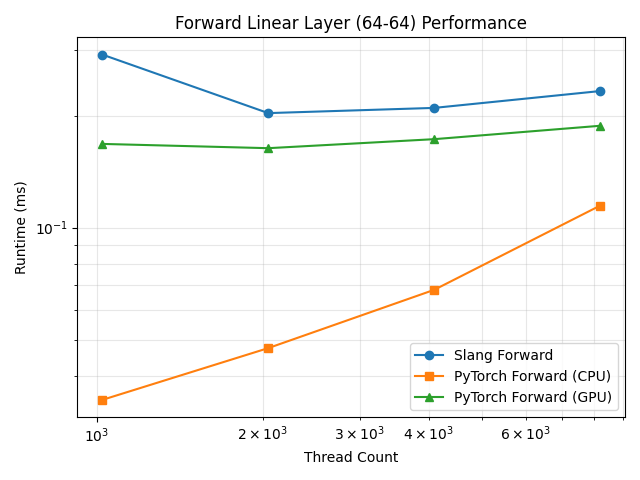
\includegraphics[width=\textwidth]{linear_forward_64x64.png}
		\caption{64x64}
		\label{fig:forward_64}
	\end{subfigure}
	\hfill
	\begin{subfigure}[b]{0.45\textwidth}
		\centering
		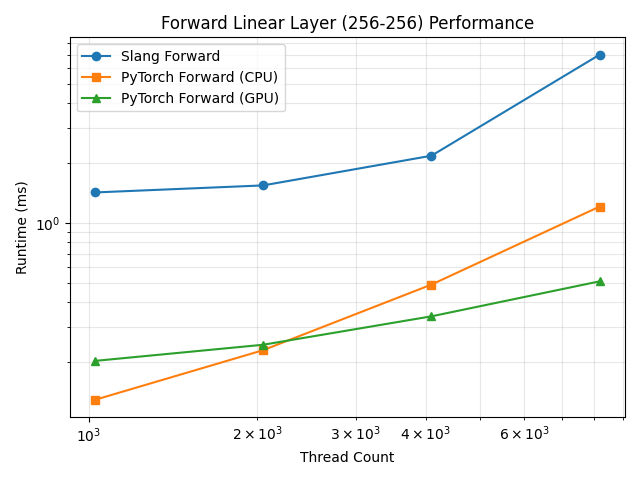
\includegraphics[width=\textwidth]{linear_forward_256x256.png}
		\caption{256x256}
		\label{fig:forward_256}
	\end{subfigure}
	\caption{Forward pass performance across different linear layer sizes. All plots show runtime (ms) vs thread count on log-log scale, comparing Slang Forward, PyTorch Forward (CPU), and PyTorch Forward (GPU).}
	\label{fig:forward}
\end{figure*}

As shown in the figure, when the linear layer size is small (64x64), the performance of Slang and PyTorch on GPU are comparable, and both are significantly slower than PyTorch on CPU. This is likely because the overhead of launching GPU kernels and the memory bandwidth bottleneck outweigh the benefits of parallelism for small linear layers. However, when the linear layer size increases to 256x256, the performance of PyTorch on GPU starts to outperform PyTorch on CPU given a large enough thread count (batch size). For comparison, the performance of the naive linear layer implementation in Slang does not improve much with increasing thread count, and it is significantly slower than PyTorch on GPU. As discussed previously, this is likely because the data-parallel implementation in Slang suffers from the memory throughput bottleneck, while PyTorch can leverage optimized matrix multiplication libraries to achieve better performance.

In Figure~\ref{fig:backward}, I also benchmark the backward pass of the linear layer.

\begin{figure*}[h]
	\centering
	\begin{subfigure}[b]{0.45\textwidth}
		\centering
		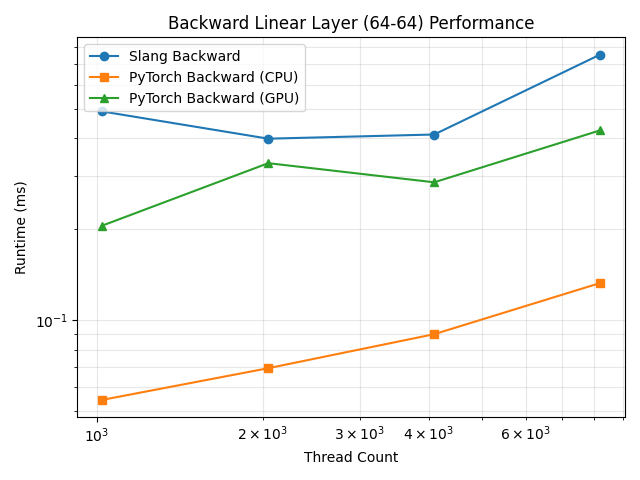
\includegraphics[width=\textwidth]{linear_backward_64x64.png}
		\caption{64x64}
		\label{fig:backward_64}
	\end{subfigure}
	\hfill
	\begin{subfigure}[b]{0.45\textwidth}
		\centering
		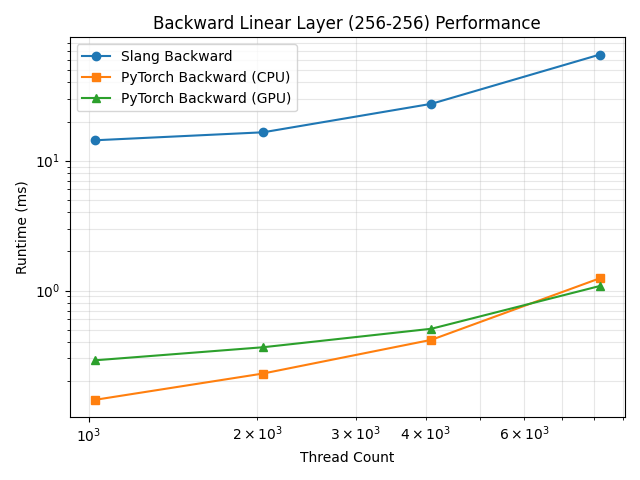
\includegraphics[width=\textwidth]{linear_backward_256x256.png}
		\caption{256x256}
		\label{fig:backward_256}
	\end{subfigure}
	\caption{Backward pass performance across different linear layer sizes. All plots show runtime (ms) vs thread count on log-log scale, comparing Slang Backward, PyTorch Backward (CPU), and PyTorch Backward (GPU).}
	\label{fig:backward}
\end{figure*}

The backward pass shows even more pronounced performance differences. Specifically, the backward kernel is only 2.14x slower than the forward kernel in PyTorch on GPU with a $256 \times 256$ linear layer and a batch size of 8192. While in Slang, the backward kernel is 7.47x slower than the forward kernel with the same linear layer size and thread count. The memory throughput bottleneck is significantly worse during backpropagation because threads must use atomic operations to accumulate gradients into shared weight and bias buffers, leading to contention and serialization. PyTorch's optimized batch matrix multiplication approach avoids these issues by reformulating the gradient computation as efficient matrix operations.

\bibliographystyle{plain}
\bibliography{references}

\end{document}
